Our database consists of perfusion MRI. During a perfusion MRI, the patient is injected by a contrast product, the gadolinium chelates. It's well known and considered that normal and pathological tissues have different way and speed absorption of the contrast product. Pathological tissues have a very specific behaviour which can be detected by our algorithm.

Figure \ref{fig:Processing_toolchain} our proposed bloc diagram.

\begin{figure*}[h]
\centering
    \includegraphics[width=\textwidth,height=5cm]{Processing_toolchain.png}
    \caption{The proposed processing tool-chain.}
    \label{fig:Processing_toolchain}
\end{figure*}



In our database and for each patient, 26 sets of 40 images have been generated, each set is corresponding to a slice of the brain. The size of each image is 128*128 pixels. Each set is used in order to retrieve the variation of pixel intensity of the slice MRI during the diffusion of contrast product.

For each slice, we generate a 128*128*40 tensor. For each pixel, we extracted a signal of 40 samples which correspond to the variation of this pixel intensity in the 40 images of 128*128 pixels. Figure \ref{fig:CourbeExample} shows the generated signals using this protocol.

\begin{figure}
\centering
    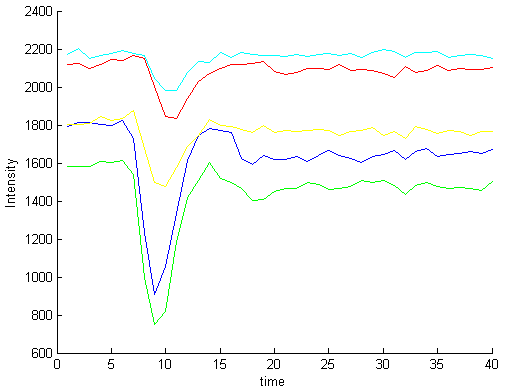
\includegraphics[scale=0.5,angle=0]{CourbeExample.png}
    \caption{Examples of signals extracted from the MRI.}
    \label{fig:CourbeExample}
\end{figure}

Figure \ref{fig:CourbeExample} shows that we obtain a hypo-signal during the diffusion of the contrast product until the intensity of the pixel come back to its original value. Our algorithm method afterwards selects a specific region of interest (ROI) on a slice and then apply a spectral clustering algorithm on those selected signals in order to cluster the different tissues of the area.




